\documentclass{article}
\usepackage{apacite}
\usepackage{hyperref}
\usepackage{multicol}
\usepackage{natbib}
\usepackage{andi}
\usepackage[utf8]{inputenc}
\usepackage{array}
\usepackage[first=0,last=9]{lcg}
\setlength{\parindent}{0pt}
\usepackage{hyperref}
\usepackage{physics}
\usepackage{soul}
\usepackage{tikz-cd}

\usepackage{courier} %% Sets font for listing as Courier.
\usepackage{listings, xcolor}
\lstset{
tabsize = 4, %% set tab space width
showstringspaces = false, %% prevent space marking in strings, string is defined as the text that is generally printed directly to the console
numbers = left, %% display line numbers on the left
commentstyle = \color{green}, %% set comment color
keywordstyle = \color{blue}, %% set keyword color
stringstyle = \color{red}, %% set string color
rulecolor = \color{black}, %% set frame color to avoid being affected by text color
basicstyle = \small \ttfamily , %% set listing font and size
breaklines = true, %% enable line breaking
numberstyle = \tiny,
}


\newcommand*{\rom}[1]{\expandafter\@slowromancap\romannumeral #1@}

\usetikzlibrary{calc,patterns,angles,quotes}
\usepackage{pgfplots}
\pgfplotsset{width=15cm,height=10cm,compat=1.9}

\pgfplotstableread{
x	y	delta-x	delta-y
-0.009	-6.3255	0.0284	0.0028
0.0611	-5.9201	0.0302	0.0019
0.2967	-5.6324	0.0375	0.0014
0.4689	-5.4092	0.0445	0.0011
0.4903	-5.2269	0.0455	0.0009
0.4822	-5.0728	0.0451	0.0008
0.5518	-4.9392	0.0485	0.0007
}{\mytable}

\begin{filecontents}{graphdata.dat}
x	y	delta-x	delta-y
-0.009	-6.3255	0.0284	0.0028
0.0611	-5.9201	0.0302	0.0019
0.2967	-5.6324	0.0375	0.0014
0.4689	-5.4092	0.0445	0.0011
0.4903	-5.2269	0.0455	0.0009
0.4822	-5.0728	0.0451	0.0008
0.5518	-4.9392	0.0485	0.0007
\end{filecontents}

\usepackage[english]{babel}
\usepackage{fancyhdr}
\usepackage{lastpage}
\pagestyle{fancy}
\fancyhf{}


\pagestyle{empty}% for cropping
\usepackage{tikz}
\usetikzlibrary{calc}
\usepackage{zref-savepos}
\usepackage{tabu}

\newcounter{NoTableEntry}
\renewcommand*{\theNoTableEntry}{NTE-\the\value{NoTableEntry}}

\newcommand*{\strike}[2]{%
  \multicolumn{1}{#1}{%
    \stepcounter{NoTableEntry}%
    \vadjust pre{\zsavepos{\theNoTableEntry t}}% top
    \vadjust{\zsavepos{\theNoTableEntry b}}% bottom
    \zsavepos{\theNoTableEntry l}% left
    \hspace{0pt plus 1filll}%
    #2% content
    \hspace{0pt plus 1filll}%
    \zsavepos{\theNoTableEntry r}% right
    \tikz[overlay]{%
      \draw
        let
          \n{llx}={\zposx{\theNoTableEntry l}sp-\zposx{\theNoTableEntry r}sp-\tabcolsep},
          \n{urx}={\tabcolsep},
          \n{lly}={\zposy{\theNoTableEntry b}sp-\zposy{\theNoTableEntry r}sp},
          \n{ury}={\zposy{\theNoTableEntry t}sp-\zposy{\theNoTableEntry r}sp}
        in
        (\n{llx}, \n{lly}) -- (\n{urx}, \n{ury})
      ;
    }% 
  }%
}

\usepackage{tikz}
\usetikzlibrary{calc}

\tikzset{
    right angle quadrant/.code={
        \pgfmathsetmacro\quadranta{{1,1,-1,-1}[#1-1]}     % Arrays for selecting quadrant
        \pgfmathsetmacro\quadrantb{{1,-1,-1,1}[#1-1]}},
    right angle quadrant=1, % Make sure it is set, even if not called explicitly
    right angle length/.code={\def\rightanglelength{#1}},   % Length of symbol
    right angle length=2ex, % Make sure it is set...
    right angle symbol/.style n args={3}{
        insert path={
            let \p0 = ($(#1)!(#3)!(#2)$) in     % Intersection
                let \p1 = ($(\p0)!\quadranta*\rightanglelength!(#3)$), % Point on base line
                \p2 = ($(\p0)!\quadrantb*\rightanglelength!(#2)$) in % Point on perpendicular line
                let \p3 = ($(\p1)+(\p2)-(\p0)$) in  % Corner point of symbol
            (\p1) -- (\p3) -- (\p2)
        }
    }
}
\pagestyle{fancy}
\fancyhf{}
\title{MDM4U1 Data Management Game Fair Report:\\Investigation of the Probability Distribution in a Pascal's Triangle}
\author{Andi Tse, Marven Wang}
\date{May 23, 2023}
\rhead{Instructor: Ms. Hung}
\lhead{Andi Tse, Marven Wang}
\chead{Game Fair Report}
\rfoot{MDM4U1}
\lfoot{Data Management}
\cfoot{Page \thepage \hspace{1pt} of \pageref{LastPage}}
\pagestyle{fancy}

 


\begin{document}

\maketitle
\tableofcontents
\newpage

\section{Game Instruction}
The player drops two coins from the top of the board (one at a time). If \textbf{both} coins land at the center of the board (Slot 5), the player wins \$15. If \textbf{both} coins land at either sides of the board (Slot 1 or Slot 9), the player wins \$100. \textbf{However, some paths were blocked so that the coins do not always have equal chances of falling in the next two slots.} A Video of the game play is attached below\footnote{\url{https://drive.google.com/file/d/10n_oc75wfgp2mhqmT-_cmTUp1paUQDnb/view?usp=sharing}}.


\begin{center}

\includegraphics[height=7cm]{Diagrams/Game Fair Board Bird View.jpg}\ \ \ \ 
\includegraphics[height=7cm]{Diagrams/Game Fair Board Pic.jpg}\ \ \ \ 
\includegraphics[height=7cm]{Diagrams/Game Fair Poster.jpg}
\end{center}



Here are the data collected over the game fair. For example, $23$ means that one coin hits Slot 2 and the other one hits Slot 3:\label{tally chart}\\
14 15 16 17 23 23 23 23 23 23 23 23 23 24 24 24 24 24 24 25 25 25 25 25 26 26 26 26 26 27 27 27 27 27 27 28 28 33 33 33 33 34 34 34 34 34 35 35 35 35 35 35 35 35 35 35 35 35 35 35 36 36 36 36 36 36 36 36 37 37 37 37 37 37 37 38 38 39 39 44 44 44 44 44 44 45 45 45 45 45 45 45 45 45 45 45 45 45 45 45 45 45 45 45 45 45 45 45 45 46 46 46 46 46 46 46 46 46 46 46 46 46 46 46 46 46 46 46 46 46 46 47 47 47 47 47 47 47 47 48 48 48 55 55 55 55 55 55 56 56 56 56 56 56 56 56 56 56 56 56 56 56 56 56 57 57 57 57 57 57 57 57 57 57 57 58 58 58 58 58 58 66 66 66 66 66 67 67 67 68 77 77 77 77 78 78 78 79 88 89 

\begin{align*}
n(1) &= 4&
n(2) &= 33&
n(3) &= 55\\
n(4) &= 81&
n(5) &= 89&
n(6) &= 66\\
n(7) &= 48&
n(8) &= 20&
n(9) &= 4
\end{align*}


\pagebreak
\section{Probabilities}
Let $n=200$ be the number of trials, both coins hitting the middle slot to be event $X$ which happens $x$ times, both coins hitting the side slots to be event $Y$ with happened $y$ times, any other cases to be event $Z$ which happened $n-x-y$ times.

\subsection{Tree Diagram}
The theoretical distribution is as followed,
\begin{center}% https://tikzcd.yichuanshen.de/#N4Igdg9gJgpgziAXAbVABwnAlgFyxMJZATgBoBGAXVJADcBDAGwFcYkRyQBfU9TXfIRQAOUgCZqdJq3acefbHgJFyABnGSGLNog7deIDIsFEA7KQDMm6Tr3zD-JUOTlyl69tn6FA5SjJWNFoyumLeDsZ+yABspAAsHiF2Bka+zqIJQTbsFuGpTirqmVKeurn2+SYo5GLxibZyKY5VyACspK31XhXNUeadWaUgpnm9zmQDJUnlTZHOrh1dunGjcyoWi4NJjT4FKHGk0UvJuy2xR1u2wqtpRKIXUw2qN3su6g-BtiM9a9W1H9ldK0Xi1yAcAUMdhFbigNqZjlDKlF2vDLuxiCC+qRUY9ZNcfjCSNiEd9ZoSFjjPrIwgTXuQ4cdopj5iiEcyiLVhGzaS0Dly0bo1Ozqup+bjBaTTlFYmKqaFJdDXqJZYCQBZgTyojVSCqhhZnpr5nzjgqkfMZdyyXTSMRLVLnBtbQKOIixkR2k7xWrTW6UOZPXKQNEaVaWmQA6rWiH7So3BGhnEfb8XI7jhYk+SPcd8aGtf67Yqw6RVMcADqlnAwAAeOGAABEAE4QNAAAhwAAsYC2AMYQLBgOBcYXIdRUZ3kAB65crNeAcBwXGn1drLYAMvQAJ4wBtDw1EdQSZ1iKcV5fAMBQRen2drzfb3e55zqQJeiwnme1huXpc39dbnfDkUxxxO+Z4dleH7ALe-4PjGKDqJMgatKBs7gT+K5-vegGHIyKG1mh14YXeAF7vBxLOqYeHAARkHQVhpEjjq2ZUTRZ50SRj77jaxzECx7YQWxmEcXBjFqGWhHAAA8swOC9gAtjAsGFlqFAluOVHzgJN4AMqMBAC7DhsYlHlRF5aSuun6UpZruqpaZUV+5lQZZBkMeYxleiB6HUfx3kti51m+kSHlIXxTn+XprmcdUbghaq0RhX5AXDvSdkUYlEkRVZKXtHFQzCBltHJQx5DuWpXq8d5rG-sRgXJqOY5et5AAKTYAEb0G1WCMLgG4thAABmLbtrgeBgAA5i2uD9WA3aKSlFCNYG5YDQ29DdsA5BcMAx7AMQAC0W11YSRlLaqK1rRtrjbbtB1HcOuVnUMF3rcA6Y3ROe2HVwx2vO5T1JC9G3Bh9X33QxZCuOJq2vVGoN3T9KWxQDthA8Aibw99v2gqd0OXW9piY+D0UuI9eOvcIROIyV-3k1dVPYypNTiYwMADTgAAUaNbTtn0I1eDZYON7Y4AAlBO0bKU+FCHk1EmtRAHVdT1OB9YNw2jf2k3TTgADuWBzYzDoyyzbOc9zPO3Vj5aC8LYsSw9JvOuWrPs1zpYwxt7282DP020LIvi5LNl+k7cuu+bHv4yDPv8-7dtB8OkOy8tpYR+7nvAHDsfW6WtuBw7JWxSn51p2bGf4xjOdHfHBfB0FqXM87Zdu2j3tWzXecB-b9fJuQuUl89LeR5nlPV37XcJ4XJOlWHqeZ5bfNY9wkgwFA43wEQoCrRAclIOoIA4BASBbQYO974gB9H0gYj2OfJ80NfiAWHfTYX7Uh-H4gcSv7vD+f0gVov936Py-kAs+b8kAbAAYgaIwCoGgKQITCBf9EDtBgcg7ekC0GIMQJTFBF8DgwPwVg1BRCn7EHgbA3BagqGxBgddAhSCaFuBAD1MAtgoAQGYG1VmIAaCdnoFAJAYBmCMEYI-eg3V2CQA4eEe+eCaG3yYYohhL8VFkDUVQzRT8wRUPMAwj+jBOowEYM1X0IB+zYFgPwkAgjhGIFEeIyR0jdDtggBAAA1kwHAtj2GcPoHATswiqFqBoeA0hF8wkMLgSohYMTQmsN0ZgkACjtQMJSWkj+uiSGpOwalBhuS0nQN0ZQuJ5Cv7kDKZEk+FSb6qFCegp+YhT41MQP3XBYhlFtPIPQ5p3S8moN6Z09RPSDHNNGYMqJ4yv5iB-nE0QMC5mhMWc0iJUyT46NmestJWyb6xLaWIK+syDkbMQEczpmTsEtM6UU65STZnVLOV0zpTyFFiCaV-fUNBjFtVMeY34liBxYBsT8-sASglr3kdc7JXzWnPJKXCqhYhEVQIGe8upz90XXMxfqZFnyoHQP8ewLhPC+ECJgEIkRYiJGHykYwGRBA2DIr6V8yZ7zWVQPmYcmZXLkW8ufjs65qyvmnPeSKqBVzUFiD2c-KV79ZUWDuagiwDyoHKovqq3BFg3nYIsLCqBuqVUGu-g0lR3yYFxDNW0i1T84jwoURYVF38HV6udXEbFKrMUeqoRYb17K9UEu-gGlVQa4g-0oFwIAA
\begin{tikzcd}[column sep={2.3em,between origins}, /tikz/column 1/.append style={nodes={anchor=base east}}]
\label{tree}
                                       &                                  &                         &                                   &                          &                                   &                          &                                   &                                                    & |[overlay]|\text{Drop the coins}             &                          &                                              &                          &                                   &                         &                                  &                         &                          \\
1^\text{st}\text{ Layer}               &                                  &                         &                                   &                          &                                   &                          &                                   &                                                    & \frac{256}{256} \arrow[ld] \arrow[rd]           &                          &                                              &                          &                                   &                         &                                  &                         &                          \\
2^\text{nd}\text{ Layer}               &                                  &                         &                                   &                          &                                   &                          &                                   & \frac{128}{256} \arrow[ld] \arrow[rd]                            &                                   & \frac{128}{256} \arrow[rd] \arrow[ld]  &                                              &                          &                                   &                         &                                  &                         &                          \\
3^\text{rd}\text{ Layer}               &                                  &                         &                                   &                          &                                   &                          & \frac{64}{256} \arrow[ld] \arrow[rd]           &                                                    & \frac{128}{256} \arrow[ld] \arrow[rd]           &                          & \frac{64}{256} \arrow[ld] \arrow[rd]                      &                          &                                   &                         &                                  &                         &                          \\
4^\text{th}\text{ Layer}               &                                  &                         &                                   &                          &                                   & \frac{32}{256} \arrow[ld] \arrow[rd]  &                                   & \frac{96}{256} \arrow[ld, Rightarrow,red] \arrow[rd, dashed,red] &                                   & \frac{96}{256} \arrow[ld] \arrow[rd]  &                                              & \frac{32}{256} \arrow[ld] \arrow[rd]  &                                   &                         &                                  &                         &                          \\
5^\text{th}\text{ Layer}               &                                  &                         &                                   &                          & \frac{16}{256} \arrow[ld] \arrow[rd]           &                          & \frac{112}{256} \arrow[ld] \arrow[rd]           &                                                    & \frac{48}{256} \arrow[ld] \arrow[rd]           &                          & \frac{64}{256} \arrow[ld] \arrow[rd]                      &                          & \frac{16}{256} \arrow[ld] \arrow[rd]           &                         &                                  &                         &                          \\
6^\text{th}\text{ Layer}               &                                  &                         &                                   & \frac{8}{256} \arrow[ld] \arrow[rd]  &                                   & \frac{64}{256} \arrow[ld] \arrow[rd]  &                                   & \frac{80}{256} \arrow[ld] \arrow[rd]                           &                                   & \frac{56}{256} \arrow[ld] \arrow[rd]  &                                              & \frac{40}{256} \arrow[ld] \arrow[rd]  &                                   & \frac{8}{256} \arrow[ld] \arrow[rd] &                                  &                         &                          \\
7^\text{th}\text{ Layer}               &                                  &                         & \frac{4}{256} \arrow[ld] \arrow[rd]           &                          & \frac{36}{256} \arrow[ld] \arrow[rd]           &                          & \frac{72}{256} \arrow[ld] \arrow[rd]          &                                                    & \frac{68}{256} \arrow[ld] \arrow[rd]          &                          & \frac{48}{256} \arrow[ld, dashed,red] \arrow[rd, Rightarrow,red] &                          & \frac{24}{256} \arrow[ld] \arrow[rd]           &                         & \frac{4}{256} \arrow[ld] \arrow[rd]          &                         &                          \\
8^\text{th}\text{ Layer}               &                                  & \frac{2}{256} \arrow[ld] \arrow[rd] &                                   & \frac{20}{256} \arrow[ld] \arrow[rd] &                                   & \frac{54}{256} \arrow[ld] \arrow[rd] &                                   & \frac{70}{256} \arrow[ld] \arrow[rd]                           &                                   & \frac{34}{256} \arrow[ld] \arrow[rd] &                                              & \frac{60}{256} \arrow[ld] \arrow[rd] &                                   & \frac{14}{256} \arrow[ld] \arrow[rd] &                                  & \frac{2}{256} \arrow[ld] \arrow[rd] &                          \\
9^\text{th}\text{ Layer}               & \frac{1}{256}                                &                         & \frac{11}{256}                                &                          & \frac{37}{256}                                &                          & \frac{62}{256}                                &                                                    & \frac{52}{256}                                &                          & \frac{47}{256}                                           &                          & \frac{37}{256}                                &                         & \frac{8}{256}                                &                         & \frac{1}{256}               \\
\begin{tabular}{@{}c@{}}Probability of \\ hitting it twice\end{tabular} & \boxed{\left(\dfrac{1}{256}\right)^2} &                         & \left(\dfrac{11}{256}\right)^2 &                          & \left(\dfrac{37}{256}\right)^2 &                          & \left(\dfrac{62}{256}\right)^2 &                                                    & \boxed{\left(\dfrac{52}{256}\right)^2} &                          & \left(\dfrac{47}{256}\right)^2            &                          & \left(\dfrac{37}{256}\right)^2 &                         & \left(\dfrac{8}{256}\right)^2 &                         & \boxed{\left(\dfrac{1}{256}\right)^2}            \\
\text{Outcome (Slot)}                         & 1^\text{st}\text{  }          &                         & 2^\text{nd}\text{  }           &                          & 3^\text{rd}\text{  }           &                          & 4^\text{th}\text{  }           &                                                    & 5^\text{th}\text{  }           &                          & 6^\text{th}\text{  }                      &                          & 7^\text{th}\text{  }           &                         & 8^\text{th}\text{  }          &                         & 9^\text{th}\text{  }     
\end{tikzcd}
\end{center}

Probability of Event $Z$ would be $1-p_1-p_2=1-\left(\frac{52}{256}\right)^{2}-\left(\frac{2}{256}\right)^{2}$

\pagebreak
\subsection{Expected Value}
\label{table}
\begin{center}
\resizebox{16cm}{!}{
\begin{tabular}{|c|c|c|c|c|}


\hline

Outcomes & \begin{tabular} {@{}c@{}} \$Prize Random \\ Variable ($X$) \end{tabular} & \begin{tabular}{@{}c@{}} Theoretical \\ Probabilities $P(X)$ \end{tabular} & \begin{tabular} {@{}c@{}}Experimental \\ Probabilities \end{tabular} & \begin{tabular} {@{}c@{}}Compared \\ Experimental to\\Theoretical,\\increased or\\decreased?\end{tabular}\\ \hline

Event $X$ & 15& $p_1=\left(\dfrac{52}{256}\right)^{2}=0.041$ & $\dfrac{6}{200}=0.03$ & $\downarrow$
\\ \hline

Event $Y$
&
100 &
$p_2=\left(\dfrac{2}{256}\right)^{2}=0.00006$
&
$\dfrac{0}{200}=0$ &
$\downarrow$
\\ \hline


Event $Z$ &0&$1-p_1-p_2=\dfrac{15707}{16384}=0.958679199219$&$\dfrac{194}{200}=0.97$&$\uparrow$\\ \hline


\multicolumn{2}{|c|}{\begin{tabular}{@{}c@{}}
    $15\left(\dfrac{52}{256}\right)^{2}+100\left(\dfrac{2}{256}\right)^{2}-1=-0.375$
\end{tabular}}
&
\begin{tabular}{@{}c@{}}
    Expected Value for\\ Theoretical Expected Value \\$E(X)=-0.375$
\end{tabular}
&
\begin{tabular}{@{}c@{}}
Expected Value for \\ experimental $E(X)=$ \\ $15(0.03)+100(0)-1=-0.55$
\end{tabular} & $\downarrow$ \\ \hline

\end{tabular}}
\end{center}




\section{Bar Graph}
The data below is taken from \ref{tally chart}. For example, data $21$ means one coin hits Slot 2 and the other one hits Slot 1. $21$ would contribute to both Slot 2 and Slot 1. Therefore, there are $2n=400$ trials for the bar graph below.  


\begin{center}
    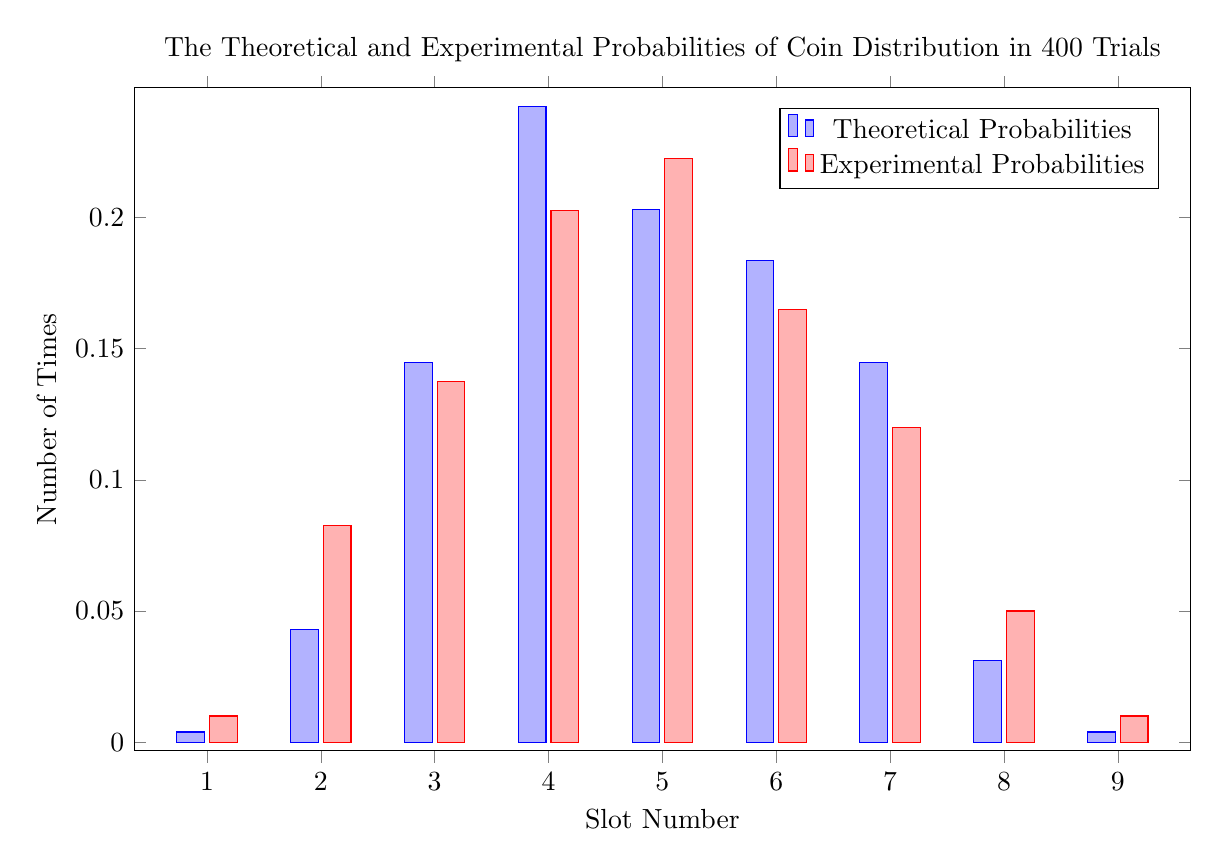
\begin{tikzpicture}
\begin{axis}[
title={The Theoretical and Experimental Probabilities of Coin Distribution in 400 Trials},
	%x tick label style={		/pgf/number format/1000 sep=},
	ylabel=Number of Times,
	xlabel=Slot Number,
	enlargelimits=0.03,
enlarge x limits=0.08,
	%legend style={at={(0.5,-0.1)}},
	legend pos=north east,
	ybar =1.8,
 ytick={0,0.05,0.10,0.15,0.20,0.25},
scaled y ticks = false,
y tick label style={/pgf/number format/fixed}
]
\addplot+ 
	coordinates {(1,0.00390625)(2,0.04296875)(3,0.14453125)(4,0.2421875)(5,0.203125)(6,0.18359375)(7,0.14453125)(8,0.03125)(9,0.00390625)};
\addplot+ 
	coordinates {(1, 0.01)(2, 0.0825)(3, 0.1375)(4, 0.2025)(5, 0.2225)(6, 0.165)(7, 0.12)(8, 0.05)(9, 0.01)};
\legend{Theoretical Probabilities,Experimental Probabilities}
\end{axis}
\end{tikzpicture}
\end{center}








\pagebreak
\section{Additional Information: Statistical Modeling}
This section models the distribution of the coins with probability models, and find the probability of having a negative experimental expected value. Assuming that the distribution of the coins follows the tree diagram \ref{tree} exactly. 



\subsection{Trinomial Distribution Over the Three Possible Outcomes}
\begin{definition}
    Given $n$ number of trials, probability of $p_1,p_2,1-p_1-p_2$ for event $X,Y,Z$ respectively, and that event $X,Y,Z$ happens $x,y,1-x-y$ times respectively. The probability of given by,
    \[P(x, y)=P(X=x, Y=y)={n\choose x}p_1^x{n-x\choose y}p_2^y\left(1-p_1-p_2\right)^{n-x-y}\]

    or in factorial notation:
    
    
    \[P(x,y)=\frac{n ! p_1^x p_2^y\left(1-p_1-p_2\right)^{n-x-y}}{x ! y !(n-x-y) !}\]
\end{definition}


Applying the Trinomial Distribution,
\[P\left(x,y\right)={n\choose x}\left(\frac{13}{64}\right)^{2x}{n-x\choose y}\left(\frac{1}{128}\right)^{2y}\left(1-\left(\frac{13}{64}\right)^{2}-\left(\frac{1}{128}\right)^{2}\right)^{n-x-y}\tag{1}\label{P(x,y)}\]
There were 6 incidences of event $X$ and 0 incidences of event $Y$ in the game fair, applying the formula gives,
\[P(6,0)=0.113175983281\]\label{P(6,0)}


\subsection{Event $X$}
Because the probability of $Y$ is so small that it becomes almost negligible, a simplification of the model \ref{P(x,y)} is to ignore Event $Y$ (Event $Y$ is \textit{ignored} but not restricted to 0). The Binomial Distribution is suitable for this modeling,

\[B_m(x)={n\choose x}\left(\frac{13}{64}\right)^{2x}\left(1-\left(\frac{13}{64}\right)^2\right)^{n-x}\]

$B_m(x)$ is the probability of both coins hitting the middle slot for $x$ times out of $n=200$ trials. 


\pagebreak
\begin{formula}
    Normal Distribution with mean of $\mu$ and standard deviation of $\sigma$ is defined by the bell curve,
    \[N(x)=\frac{1}{\sigma \sqrt{2 \pi}} e^{-\frac{1}{2}\left(\frac{x-\mu}{\sigma}\right)^2}\]
\end{formula}

Binomial Approximation is applicable here because  

\begin{align*}
\mu=np_1&=n\left(\frac{52}{256}\right)^{2}=8.251953125>5\\np_1'&=n\left(1-\left(\frac{52}{256}\right)^{2}\right)=191.748046875>5\\
\sigma&=\sqrt{np_1p_1'}=0.0224423538951\\
\therefore N_m&=\frac{1}{0.0224\sqrt{2\pi}}e^{-\frac{1}{2}\left(\frac{x-8.2520}{0.0224}\right)^2}
\end{align*}



Binomial Distribution is chosen over Binomial Approximation for accuracy purposes. 


\subsection{Event $Y$}
Similarly, $p_2=\left(\dfrac{2}{256}\right)^2$, middle slots were hit $x$ times. Now there are only $n-x$ trials remaining, using Binomial Distribution:

\[B_s(x,y)={n-x\choose y}\left(\left(\dfrac{2}{256}\right)^{2}\right)^y\left(1-\left(\dfrac{2}{256}\right)^2\right)^{n-x-y}\]

$B_s(x)$ is the probability of both coins hitting the side slot for $x$ times out of $n=200$ trials.\\
Binomial Approximation is not applicable because,

\begin{align*}
np_2&=n\left(\frac{2}{256}\right)^{2}=0.01220703125<5\\np_2'&=n\left(1-\left(\frac{2}{256}\right)^{2}\right)=199.987792969>5
\end{align*}




\subsection{Probability of Players Losing Money}

The player makes $15x+100y$ dollars with event $X$ triggered $x$ times, and event $Y$ triggered $y$ times.
\begin{align*}
    15x+100y&<n\\
    x&<\frac{n-100y}{15}\\
    x&<\frac{n}{15}\tag{Maximizing $x$}\\
    y&<\frac{n-15x}{100}
\end{align*}
Add all combinations of $x,y$ with $15x+100y<n$ using $P(x,y)$ from \ref{P(x,y)} to evaluate the probability of negative profit,
\[\sum_{x=0}^{\ceiling{\dfrac{n}{15}}-1} 
 \sum_{y=0}^{\ceiling{\dfrac{n-15x}{100}}-1}P\left(x,y\right)=0.952885338455\label{negative m}\]


\subsection{Expected Value Using $P(x,y)$}
Every possible case are added to evaluate the expected value,

\[
    \sum_{x=0}^{n}\sum_{y=0}^{n-x}\left(\left(15x+100y\right)P\left(x,y\right)\right)-200=-75
\]
which matches the expected value from table \ref{table}, $200(-0.375)=-75$

\subsection{Full Probability Distribution Over Profit}
\subsubsection{Derivation of $P(m)$}


$P(m)$ is derived by modifying formula \ref{P(x,y)}, using $15x+100y=n+m$ where $m$ is the money that the player earns in total. For example, if the player hits the middle slot exactly 8 times and side slots 0 times, they earn $8\cdot \$15+0\cdot \$100=\$120$, and their profit is $\$120-\$200=-\$80$ due to the $\$1$ fee for every game. Therefore, the formula $P(m)$ is derived for the probability of the player profiting $\{m\in\mathbb Z|-200\leq m\leq 19800\}$ dollars out of the $n$ games,

\begin{align*}
    15x+100y&=n+m\\
    y&=\frac{n+m-15x}{100}\\
\end{align*}
Substitute this into the formula \ref{P(x,y)} would gives,
\begin{align*}
    P\left(x,\frac{n+m-15x}{100}\right)={n\choose x}\left(\frac{13}{64}\right)^{2x}{n-x\choose \frac{n+m-15x}{100}}\left(\frac{1}{128}\right)^{\frac{n+m-15x}{50}}\left(1-\left(\frac{13}{64}\right)^{2}-\left(\frac{1}{128}\right)^{2}\right)^{n-x-\frac{n+m-15x}{100}}
\end{align*}
Because $x$ can take value from $0$ to $\floor{\frac{n+m}{15}}$, we need to sum up all $P(x,y)$ that satisfy the condition of $0\leq x,y$ and $x+y\leq 200$ and $15x+100y=n+m$. In order to secure integer solutions, 
\begin{align*}
    15x+100y&=n+m\\
    100y&=n+m-15x\\
    n+m-15x&\equiv 0\pmod{100}
\end{align*}

We can arrive at the conclusion that 
\[P\left(m\right)=\sum_{\substack{x=0\\ \operatorname{mod}(n+m-15x,100)=0}}^{\floor{\frac{n+m}{15}}}{n\choose x}\left(\frac{13}{64}\right)^{2x}{n-x\choose \frac{m+n-15x}{100}}\left(\frac{1}{128}\right)^{\frac{m+n-15x}{50}}\left(\frac{15707}{16384}\right)^{n-x-\frac{m+n-15x}{100}}\tag{2}\label{P(m)}\]

\subsubsection{Java Implementation}
Because Desmos is unable to include conditions in Sigma notation, a Java program was written to evaluate $P(m)$ for all $m\in\{m\in\mathbb{Z}|-200\leq m\leq 19800\}$


\begin{lstlisting}[language = Java , frame = trBL , firstnumber = last , escapeinside={(*@}{@*)}]
// Author: Andi Tse
import java.util.*;
import java.io.*;
import java.lang.*;
import java.math.*;

public class GameFairCalculation {
	public static final int n = 200;

	public static void main(String[] args) throws IOException {
		File moneyFile = new File("Game Fair Probability Distribution Over Money.txt");
		PrintWriter fw = new PrintWriter(moneyFile);
		BigDecimal[] p = new BigDecimal[20002];

		for (int m = -200; m <= 19800; m++) {
			if (P(m).equals(new BigDecimal(0)))
				continue;
			p[m + 200] = P(m);
		}

		for (int m = -200; m <= 19800; m++) {
			if (p[m + 200] == null || p[m + 200].equals(new BigDecimal(0)))
				continue;
			fw.print("\\left(" + m + ", ");
			String s = String.valueOf(p[m + 200]);
			if (s.contains("E")) {
				s = s.substring(0, s.indexOf("E")) + "\\cdot 10^{" + s.substring(s.indexOf("E") + 1, s.length()) + "}";
			}
			fw.print(s);
			fw.println("\\right)");
		}
		fw.close();

		BigDecimal a = new BigDecimal(0);
		for (int m = -200; m < 0; m++) {
			if (p[m + 200] == null)
				continue;
			a = a.add(p[m + 200]);
		}
		System.out.println("P(m < 0) = " + a);
		a = new BigDecimal(0);
		for (int m = -200; m < 19800; m++) {
			if (p[m + 200] == null)
				continue;
			a = a.add(p[m + 200]);
		}
		System.out.println("P(all m) = " + a);

	}

	public static BigDecimal P(int x, int y) {
		return c(n, x).multiply(new BigDecimal(Math.pow(52.0 / 256, 2 * x)).multiply(c(n - x, y).multiply(
				new BigDecimal(Math.pow(1.0 / 128, 2 * y) * Math.pow(1 - Math.pow(52.0 / 256, 2)- 
						Math.pow(1.0 / 128,2),n - x - y)))));
	}

	public static BigDecimal P(int m) {

		BigDecimal a = new BigDecimal(0);
		for (int x = 0; x <= (n + m) / 15; x++) {
			if ((n + m - 15 * x) % 100 == 0) {
				a = a.add(c(n, x)
						.multiply(new BigDecimal(Math.pow(52.0 / 256, 2 * x)).multiply(c(n - x, (m + n - 15 * x) / 100)
								.multiply(new BigDecimal(Math.pow(1.0 / 128, (m + n - 15 * x) / 50.0)
										* Math.pow(1 - Math.pow(52.0 / 256, 2) - Math.pow(1.0 / 128, 2),
												n - x - (m + n - 15 * x) / 100.0))))));
			}
		}
		return a;
	}

	public static BigDecimal c(final int N, final int K) {
		// returns N choose K in BigDecimal
		BigInteger ret = BigInteger.ONE;
		for (int k = 0; k < K; k++) {
			ret = ret.multiply(BigInteger.valueOf(N - k)).divide(BigInteger.valueOf(k + 1));
		}
		return new BigDecimal(ret);
	}
}
\end{lstlisting}

The BigDecimal data type was chosen over the double data type for higher precision. The program calculates the probability of every possible profit $m$ by the player and stores in the txt file, which can be accessed here\footnote{\url{https://drive.google.com/file/d/1kBNWo8XWLyiEc9TjvVEXgateX26_UnDV/view?usp=share_link}}. The probability distribution graph can be accessed here\footnote{\url{https://www.desmos.com/calculator/nsgkph1xhd}}. The program outputs to the console
\begin{align*}
    P(m < 0) = 0.95288533845462508395
\end{align*}
Which confirms the answer from \ref{negative m}. The program also outputs to the console
\begin{align*}
    P(\text{all }m) = 1.000000000000000033427
\end{align*}
Which is reasonably close to 1. The players profited -\$110 in the game fair, $P(-110)=0.113175983281$ which confirms the answer from \ref{P(6,0)}. Errors are often better represented in absolute differences, our experimental player's profit differed $\left| -110-(-75)\right| =35$ from theoretical profit,
\begin{align*}
&P\left(\left|m_\text{experimental}-m_\text{theoretical}\right|\ge 35\right)\\
=\ &P(m\leq -110\cup m\ge -40)\\
=\ &\sum_{m=-200}^{-110}P(m)+\sum_{m=-40}^{19800}P(m)\\
=\ &0.489957215021032
\end{align*}
Therefore it is almost $50\%$ chance of falling $\$35$ or more from theoretical profit, having profit of $-110$ is acceptable.


\subsection{Probability of Experimental Expected Value \\Falls Within the Range Required}
The expected value of the game was instructed to fall between $-\$0.2$ and $-\$0.4$ inclusive,
\begin{align*}
    -0.4&\leq E(X)\leq -0.2\\
    -80&\leq m\leq -40
\end{align*}
The probability is given by
\[P\left(-0.4\leq E_\text{experimental}(X)\leq -0.2\right)=\sum_{m=-80}^{-40}P(m)=0.3756218813838177\]


\pagebreak
\section{Conclusion \& Reflection}
Looking at the bar graph, overall the experiment matches the theory. The only significant contradiction is that the side slots had noticeable more hits than it is in theory. One possible explanation is that while the coin goes down the board, the horizontal movement is not completely stopped by the board. That means that if the coin starts moving towards the sides in the beginning, it is more likely to continue to move towards the sides, which is not desired. We expected to earn $\$75$ but we earned $\$110$ so yay. 

There are three major strengths in the game:
\begin{enumerate}
    \item The game was successful given that the theoretical expected value of $-0.375$ falls between $-0.4$ and $-0.2$
    \item It is almost guaranteed that the player would loose money, HAHA, with a chance of $95.29\%$
    \item The trick to block the paths is almost unnoticeable. In fact, no one has ever noticed it
\end{enumerate}
Despite Andi's and Marven's desperate hard work, there are two major drawbacks:
\begin{enumerate}
    \item The blocking technique does not work 100\% of the time. It was noticed that the coins passed the blocked path several times during the game fair
    \item The game has a high standard deviation, there is only $37.56\%$ of the time that the experimental expected value will fall within the required range
\end{enumerate}
What did we learn from the game fair? Well Andi learned that theorists cannot survive without engineers, and that he should be more deliberate before spending an entire week on a report which is meant to take 30 minutes (\LaTeX\ ahhhhhhhhh). Marven learned that he should never use a black pen to draw on a black cardboard because no one can see it (cough cough we had to remake the poster). Gary learned that Math is very useful in life, in our first design we are using nails and adjusting their intervals to trick the paths, which involves TONS of Geometry. 

\begin{figure}[h]
    \centering
    
\includegraphics[width=12cm]{Diagrams/Game Fair first design bg removed.png}
    \caption{First Design}
\end{figure}


\pagebreak
\begin{figure}
    \centering
    
\includegraphics[width=16cm]{Diagrams/ango.png}
    \caption{Lord Ango, Mascot of Bayview Math Club}
    \label{fig:my_label}
\end{figure}





\end{document}